\documentclass[12pt,epsf,psfig,graphics]{article}             
\textwidth = 6.5in
\textheight = 9.05in
\topmargin 0.0in
\oddsidemargin 0.0in
\evensidemargin 0.0in

% set it so that subsubsections have numbers and they
% are displayed in the TOC (maybe hard to read, might want to disable)

\usepackage[T1]{fontenc}
\usepackage{mathptmx}

\usepackage{graphics}
\usepackage{pifont}
\setcounter{secnumdepth}{3}
\setcounter{tocdepth}{3}

% define widow protection 
        
\def\widow#1{\vskip #1\vbadness10000\penalty-200\vskip-#1}

% define a little section heading that doesn't go with any number

\def\littlesection#1{
\widow{2cm}
\vskip 0.5cm
\noindent{\bf #1}
\vskip 0.1cm
\noindent
}

% A paraphrase mode that makes it easy to see the stuff that shouldn't
% stay in for the final proposal

\newdimen\tmpdim
\long\def\paraphrase#1{{\parskip=0pt\hfil\break
\tmpdim=\hsize\advance\tmpdim by -15pt\noindent%
\hbox to \hsize
{\vrule\hskip 3pt\vrule\hfil\hbox to \tmpdim{\vbox{\hsize=\tmpdim
\def\par{\leavevmode\endgraf}
\obeyspaces \obeylines 
\let\par=\endgraf
\bf #1}}}}}

\renewcommand{\baselinestretch}{1.2}    % must go before the begin of doc
\newtheorem{principle}{Principle}
\newtheorem{definition}{Definition}
\newtheorem{define}{Definition}
% go with the way that CC sets the margins

\usepackage{listings}

\usepackage{color}

\definecolor{javared}{rgb}{0.6,0,0} % for strings
\definecolor{javagreen}{rgb}{0.25,0.5,0.35} % comments
\definecolor{javapurple}{rgb}{0.5,0,0.35} % keywords
\definecolor{javadocblue}{rgb}{0.25,0.35,0.75} % javadoc

\newcommand*\yes{\item[\Checkmark]}
\newcommand*\yesplus{\item[\Checkmark$^{+}$]}
\newcommand*\yesminus{\item[\Checkmark$^{-}$]}

\newcommand*\no{\item[\small{\XSolidBrush}]}

\begin{document}

\lstset{language=Java,
basicstyle=\ttfamily,
keywordstyle=\color{javapurple}\bfseries,
stringstyle=\color{javared},
commentstyle=\color{javagreen},
morecomment=[s][\color{javadocblue}]{/**}{*/},
%numbers=left,
numberstyle=\scriptsize\color{black},
stepnumber=1,
numbersep=7pt,
tabsize=4,
showspaces=false,
showstringspaces=false}

% handle widows appropriately
\def\widow#1{\vskip #1\vbadness10000\penalty-200\vskip-#1}

\begin{center}

CMPSC 440: Operating Systems\\
Examination Two\\
%Saturday December 11, 2004 \\

\end{center}

\noindent
Answer the five questions that are listed on the following pages.  You must provide answers to these questions on a
separate sheet of paper.  Please develop responses that clearly express your ideas in the most succinct manner possible.
You are not permitted to complete this examination in conjunction with any of your classmates.  Furthermore, you cannot
consult any outside references during this examination.  If you have questions concerning the following problems, then
please visit my office during the examination period.  If you leave the classroom to take the exam, then you are
responsible for checking the white board for status updates.

%\mbox{} \newline
%\mbox{} \newline

\begin{enumerate}
  
\item ({\bf 10 Points}) The memory management unit (MMU) of an operating system controls what parts of a program are in
  memory and how those programs parts are accessed.  Answer the following questions about basic memory management
  operations and their trade-offs.
  
  \begin{enumerate}
          
  \item ({\bf 2 Points}) Many computers have both RAM and ROM.  What is the meaning of these two terms?  How does a
    computer operating system use both RAM and ROM?

  \item ({\bf 5 Points}) It is possible to divide up the computer's memory into address spaces.  What is an address
    space?  What does it mean if an address space is dynamically relocatable? How could the MMU use base and limit
    registers to support dynamic relocation?   

  \item ({\bf 3 Points}) The majority of modern operating systems support both virtual and physical memory.  After
    clearly defining both of these types of memory, please state which one is faster and explain why this is the case.
    Why does an OS support both of these?
    
  \end{enumerate}
        
\newpage

% \begin{figure}[t]
%   \centering
%   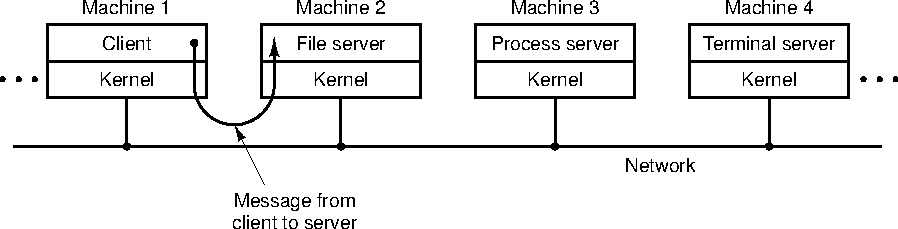
\includegraphics{fig1-27}
%   \caption{Client-Server Communication Involving the Client, a Server, and the Kernel.}
%   \label{fig:clientserver}
% \end{figure}
% 
\item ({\bf 10 Points}) It is important for the memory management unit (MMU) to be able to track the memory that is
  currently free.  Answer the following questions about managing free memory.

  \begin{enumerate}
          
  \item ({\bf 6 Points}) Suppose that the memory manager keeps a linked list of allocated and free segments.  Next,
    assume that the MMU tracks the following information for each unit of the memory; in this notation $P$
    denotes ``Process'' and $H$ stands \mbox{for ``Hole''}.

    \begin{itemize}
      \item The type marker, $T \in \{P, H\}$
      \item The start location, $S$
      \item The length of the unit, $L$
    \end{itemize}

    Using the aforementioned information that is tracked for each allocation unit, please clearly explain how the
    following memory allocation algorithms would work.

    \begin{enumerate}
      \item ({\bf 2 Points}) First fit
      \item ({\bf 2 Points}) Best fit
      \item ({\bf 2 Points}) Worst fit
      % \item ({\bf 2 Points}) Quick fit
    \end{enumerate}

  \item ({\bf 4 Points}) The memory manager should use an efficient algorithm to allocate a program to a free location in
    memory.  What is the worst-case time complexity of the first fit and best fit algorithms?  Which, if any, of these
    two algorithms is likely to be faster?

  \end{enumerate}

  \newpage

\item ({\bf 10 Points}) An operating system's memory manager often segments the memory into pages.  Answer the following
  questions about memory pages and page replacement algorithms.

  \begin{enumerate}

    \item ({\bf 2 Points}) What is a page fault? What does an operating system do when one occurs?

    \item ({\bf 2 Points}) The optimal page replacement algorithm is the ``gold standard'' by which other page
      replacement algorithms are judged.  How does this algorithm work? 

    \item ({\bf 4 Points}) Page replacement algorithms can use two bits to determine which page should be replaced.
      These bits, $R$ and $M$, have the following meanings:

      \begin{itemize} 
        \item $R$: the page was referenced 
        \item $M$: the page was modified
      \end{itemize}
  
    The not recently used (NRU) algorithm removes a page at random from the lowest-numbered non-empty class, with the
    four classes having the following names:

    \begin{itemize}
      \item Class 0
      \item Class 1
      \item Class 2
      \item Class 3
    \end{itemize}
    
    Using the $R$ and $W$ bits in your response, what is the meaning of these four classes?

    \item ({\bf 2 Points}) One of the aforementioned classes contains an entity known at the VIP.  What is the meaning
      of this term? What does the NRU algorithm do with these VIPs?

  \end{enumerate}

  \newpage
  
\item ({\bf 10 Points}) An operating system normally provides a file system that supports the persistent storage of
  data.  Answer the following questions about the creation and use of file systems.

  \begin{enumerate}

    \item ({\bf 4 Points}) Operating systems commonly support both sequential-access and random-access files.  What is
      the meaning of these two terms?  What type of file would a database management system use to store its contents?
      Why?

    \item ({\bf 4 Points}) A file system often supports navigation of directories with both relative and absolute path
      names.  What is the meaning of these two terms?  Please give an example of each path type and explain what
      indicates that the path is either relative or absolute.

    \item ({\bf 2 Points})  The following line is excerpted from an {\tt /etc/fstab} file on a Linux workstation.  What
      is the meaning of these two lines? At minimum, your response to this question should clearly explain the meaning
      of the terms {\tt /dev/sda1} and {\tt ext4}. \\

      \hspace*{-.75in}
      \vspace*{1in}
      \begin{minipage}{4in}
        \begin{verbatim}
        # / was on /dev/sda1 during installation
        UUID=5f006f4b-ff6c-4d12-9e78-a3540f33339e / ext4 errors=remount -ro 0 1
        \end{verbatim}
      \end{minipage}

  \end{enumerate}

  \newpage

  \begin{figure}[p]
    \centering
    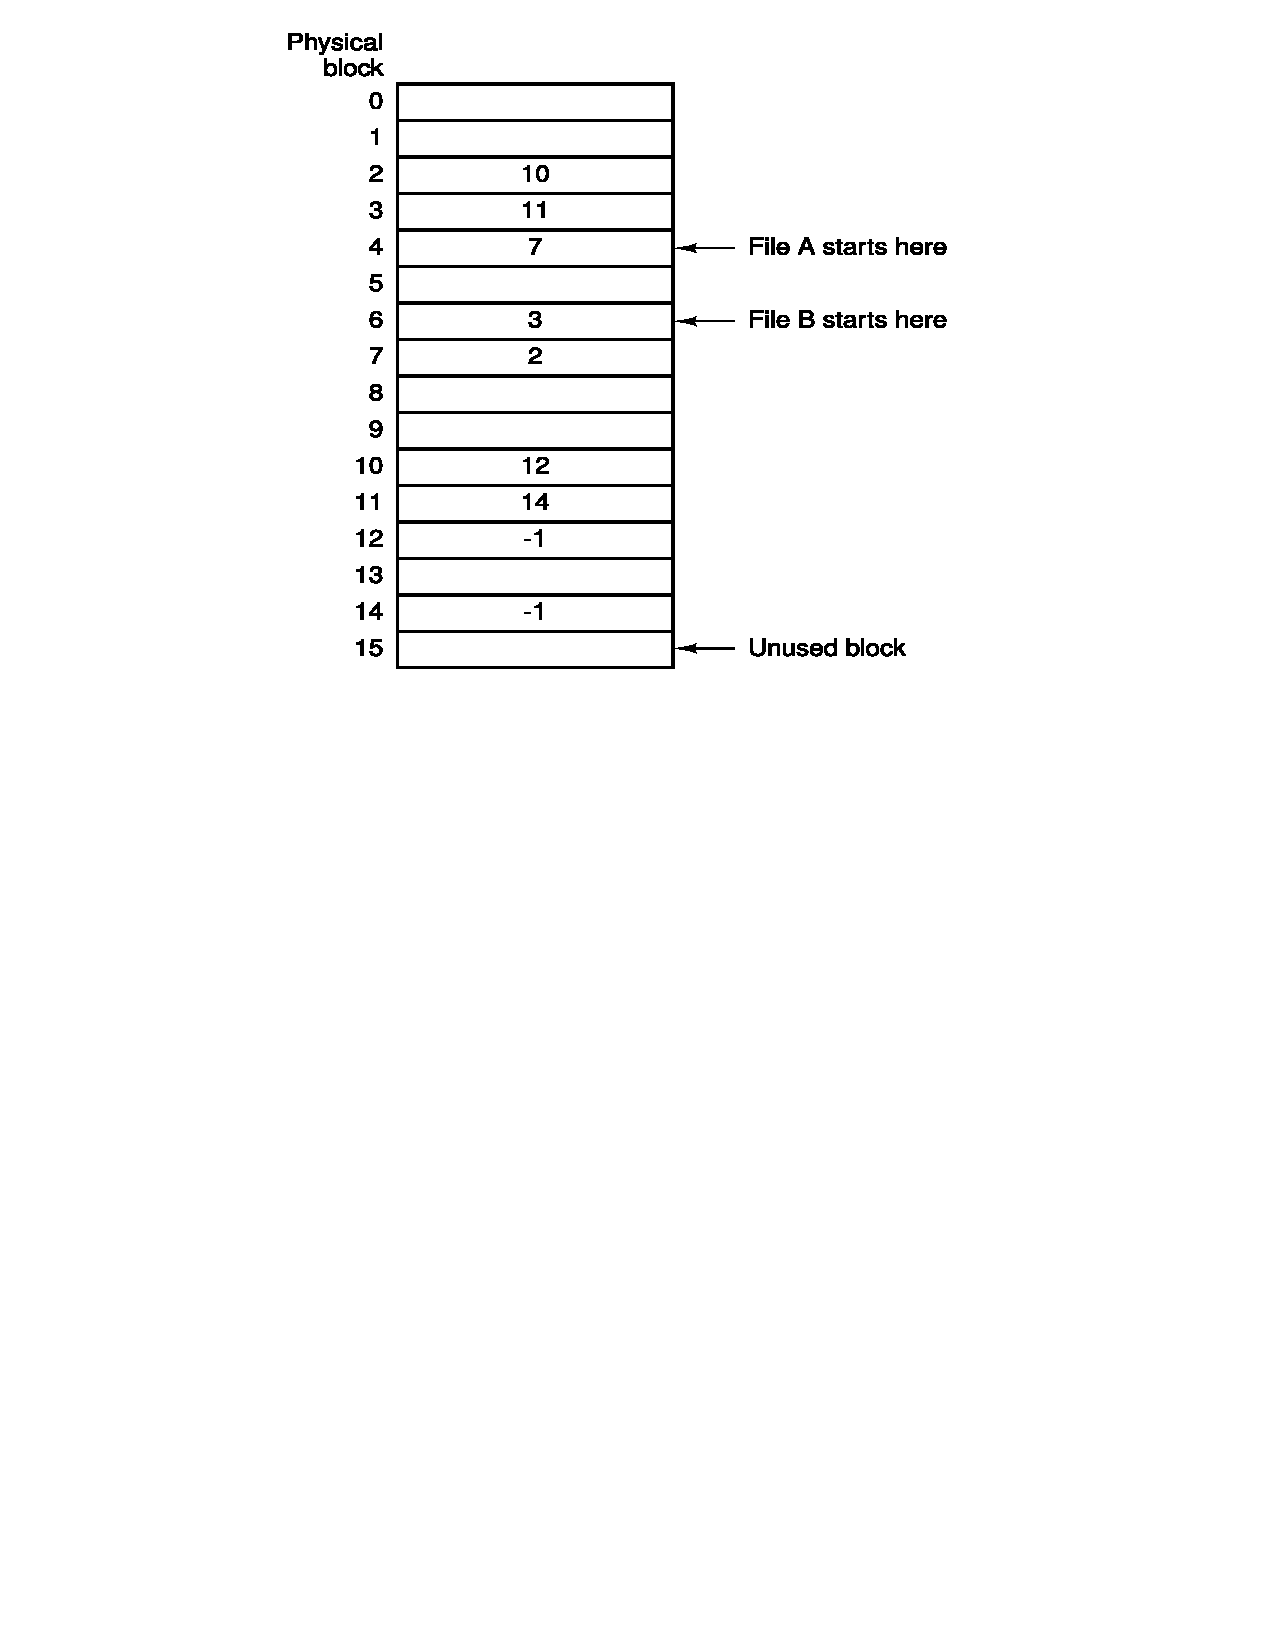
\includegraphics{fig412}
    \vspace*{-6.75in}
    \caption{A Structure for File Management.}
    \label{fig:fat}
  \end{figure}

\item ({\bf 10 Points}) The file system must have an efficient implementation of files and directories that supports
  rapid creation, deletion, and location.  Answer the following questions about file system implementation and
  the use of disk drives.

\begin{enumerate}

  \item ({\bf 5 Points}) Figure~\ref{fig:fat} shows one example of a structure that a file system can use to manage
    files.  What is the name of this structure? How does a file system use this structure to find files?  What are the
    drawbacks associated with this approach?

  \item ({\bf 3 Points}) Certain file systems, such as NTFS, provide support for journaling.  What is a
    journaling file system?  What are the benefits and drawbacks associated with journals?

  \item ({\bf 2 Points}) It is possible to have a file system run on a solid-state drive (SSD).  What is an SSD?  What
    are the benefits associated with the use of SSDs? 

\end{enumerate}

\end{enumerate}

\end{document}

